\documentclass[12pt]{beamer}
\usepackage{../Estilos/BeamerMAF}
%Sección para el tema de beamer, con el theme, usercolortheme y sección de footers
\usetheme{CambridgeUS}
\usecolortheme{beaver}
%\useoutertheme{default}
\setbeamercovered{invisible}
% or whatever (possibly just delete it)
\setbeamertemplate{section in toc}[sections numbered]
\setbeamertemplate{subsection in toc}[subsections numbered]
\setbeamertemplate{subsection in toc}{\leavevmode\leftskip=3.2em\rlap{\hskip-2em\inserttocsectionnumber.\inserttocsubsectionnumber}\inserttocsubsection\par}
\setbeamercolor{section in toc}{fg=blue}
\setbeamercolor{subsection in toc}{fg=blue}
\setbeamercolor{frametitle}{fg=blue}
\setbeamertemplate{caption}[numbered]

\setbeamertemplate{footline}
\beamertemplatenavigationsymbolsempty
\setbeamertemplate{headline}{}


\makeatletter
\setbeamercolor{section in foot}{bg=gray!30, fg=black!90!orange}
\setbeamercolor{subsection in foot}{bg=blue!30!yellow, fg=red}
\setbeamercolor{date in foot}{bg=black, fg=white}
\setbeamertemplate{footline}
{
  \leavevmode%
  \hbox{%
  \begin{beamercolorbox}[wd=.333333\paperwidth,ht=2.25ex,dp=1ex,center]{section in foot}%
    \usebeamerfont{section in foot} \insertsection
  \end{beamercolorbox}%
  \begin{beamercolorbox}[wd=.333333\paperwidth,ht=2.25ex,dp=1ex,center]{subsection in foot}%
    \usebeamerfont{subsection in foot}  \insertsubsection
  \end{beamercolorbox}%
  \begin{beamercolorbox}[wd=.333333\paperwidth,ht=2.25ex,dp=1ex,right]{date in head/foot}%
    \usebeamerfont{date in head/foot} \insertshortdate{} \hspace*{2em}
    \insertframenumber{} / \inserttotalframenumber \hspace*{2ex} 
  \end{beamercolorbox}}%
  \vskip0pt%
}
\makeatother\newlength{\depthofsumsign}
\setlength{\depthofsumsign}{\depthof{$\sum$}}
\newcommand{\nsum}[1][1.4]{% only for \displaystyle
    \mathop{%
        \raisebox
            {-#1\depthofsumsign+1\depthofsumsign}
            {\scalebox
                {#1}
                {$\displaystyle\sum$}%
            }
    }
}
\def\scaleint#1{\vcenter{\hbox{\scaleto[3ex]{\displaystyle\int}{#1}}}}
\def\bs{\mkern-12mu}






\makeatletter
\setbeamertemplate{footline}
{
  \leavevmode%
  \hbox{%
  \begin{beamercolorbox}[wd=.333333\paperwidth,ht=2.25ex,dp=1ex,center]{section in foot}%
    \usebeamerfont{section in foot} \insertsection
  \end{beamercolorbox}%
  \begin{beamercolorbox}[wd=.333333\paperwidth,ht=2.25ex,dp=1ex,center]{subsection in foot}%
    \usebeamerfont{subsection in foot}  \insertsubsection
  \end{beamercolorbox}%
  \begin{beamercolorbox}[wd=.333333\paperwidth,ht=2.25ex,dp=1ex,right]{date in head/foot}%
    \usebeamerfont{date in head/foot} \insertshortdate{} \hspace*{2em}
    \insertframenumber{} / \inserttotalframenumber \hspace*{2ex} 
  \end{beamercolorbox}}%
  \vskip0pt%
}
\makeatother
\date{13 de octubre de 2021}

\title{\large{Ec. Helmholtz en coordenadas parabólicas}}
\subtitle{Tema 2 - Primeras técnicas de solución}
\author{M. en C. Gustavo Contreras Mayén}

\begin{document}
\maketitle
\fontsize{14}{14}\selectfont
\spanishdecimal{.}

\section*{Contenido}
\frame{\tableofcontents[currentsection, hideallsubsections]}

\section{La ecuación de Helmholtz}
\frame{\tableofcontents[currentsection, hideothersubsections]}
\subsection{Enunciado del ejercicio}

\begin{frame}
\frametitle{Planteamiento del ejercicio}
Demostrar que la ecuación de Helmholtz:
\begin{align}
\laplacian{\psi} + k^{2} \, \psi = 0
\label{eq:ecuacion_Helmholtz}
\end{align}
es separable en un sistema de coordenadas parabólicas.
\end{frame}
\begin{frame}
\frametitle{Elementos necesarios}
Como el enunciado lo indica, debemos de ocupar el sistema coordenado parabólico, \pause por lo que presentaremos los elementos que se van a ocupar, ya que en algún momento se han trabajado.
\end{frame}
\begin{frame}
\frametitle{Elementos necesarios}
En algún otro ejercicio que especifique un sistema coordenado distinto que no hayamos trabajo, deberás de construir el operador diferencial necesario, y como sabemos, se requieren los correspondientes factores de escala, que deberán de estar desarrollados.
\end{frame}

\subsection{Operador Laplaciano}

\begin{frame}
\frametitle{El Laplaciano}
El Laplaciano en coordenadas parabólicas $(\varepsilon, \eta, \varphi)$ es:
\begin{align*}
\laplacian{\psi} &= \dfrac{1}{(\varepsilon^{2} + \eta^{2}) \, \varepsilon} \, \pdv{\varepsilon} \left( \varepsilon \, \pdv{\psi}{\varepsilon} \right) + \\[0.5em]
&+ \dfrac{1}{(\varepsilon^{2} + \eta^{2}) \, \eta} \, \pdv{\eta} \left( \eta \, \pdv{\psi}{\eta} \right) + \dfrac{1}{\varepsilon^{2} \, \eta^{2}} \, \pdv{\psi}{\varphi}
\end{align*}
\end{frame}

\subsection{Separación de variables}

\begin{frame}
\frametitle{El método de separación de variables}
El método de separación de variables funciona cuando:
\pause
\setbeamercolor{item projected}{bg=red!70!black,fg=yellow}
\setbeamertemplate{enumerate items}[circle]
\begin{enumerate}[<+->]
\item En la expresión no hay términos con derivadas parciales mixtas.
\item La función solución que propongamos es un producto de funciones de una sola variable:
\pause
\begin{align*}
\psi = E(\varepsilon) \, H(\eta) \, F(\varphi)
\end{align*}
\end{enumerate}
\end{frame}
\begin{frame}
\frametitle{Ocupando la solución}
Sustituimos la solución en la ecuación diferencial (\ref{eq:ecuacion_Helmholtz}):
\pause
\begin{align*}
&\dfrac{H(\eta) \, F(\varphi)}{(\varepsilon^{2} {+} \eta^{2}) \, \varepsilon} \, \dv{\varepsilon} \left( \varepsilon \, \dv{E(\varepsilon)}{\varepsilon} \right) + 
\dfrac{E(\varepsilon) \, F(\varphi)}{(\varepsilon^{2} {+} \eta^{2}) \, \eta} \, \dv{\eta} \left( \eta \, \dv{H(\eta)}{\eta} \right) + \\[0.5em]
&+ \dfrac{E(\varepsilon) \, H(\eta)}{\varepsilon^{2} \, \eta^{2}} \, \dv[2]{F(\varphi)}{\varphi} + k^{2} \, E(\varepsilon) \, H(\eta) \, F(\varphi) = 0
\end{align*}
\pause
Tenemos una ecuación con derivadas ordinarias, ya que cada función depende de una sola variable independiente.
\end{frame}
\begin{frame}
\frametitle{Dividiendo entre la solución}
Dividimos la expresión anterior entre $E(\varepsilon) \, H(\eta) \, F(\varphi)$:
\pause
\begin{align*}
&\dfrac{1}{E \, \varepsilon \, (\varepsilon^{2} {+} \eta^{2})} \, \dv{\varepsilon} \left( \varepsilon \, \dv{E}{\varepsilon} \right) + 
\dfrac{1}{H \, \eta \, (\varepsilon^{2} {+} \eta^{2})} \, \dv{\eta} \left( \eta \, \dv{H}{\eta} \right) + \\[0.5em]
&+ \dfrac{1}{ F \,  \varepsilon^{2} \, \eta^{2}} \, \dv[2]{F}{\varphi} + k^{2} = 0    
\end{align*}
\pause
Multiplicamos toda la expresión por: $\varepsilon^{2} \, \eta^{2}$.
\end{frame}
\begin{frame}
\frametitle{Expresión obtenida}
\pause
\begin{align*}
&\dfrac{\varepsilon \, \eta^{2}}{E \, (\varepsilon^{2} {+} \eta^{2})} \, \dv{\varepsilon} \left( \varepsilon \, \dv{E}{\varepsilon} \right) + 
\dfrac{\varepsilon^{2} \, \eta}{H \, (\varepsilon^{2} {+} \eta^{2})} \, \dv{\eta} \left( \eta \, \dv{H}{\eta} \right) + \\[0.5em]
&+ \dfrac{1}{F} \, \dv[2]{F}{\varphi} + k^{2} \, \varepsilon^{2} \, \eta^{2} = 0
\end{align*}
\pause
El penúltimo sumando solo depende de la variable $\varphi$, por lo podemos separar el término de la siguiente forma:
\end{frame}
\begin{frame}
\frametitle{Primera constante de separación}
\pause
\begin{align*}
&\dfrac{\varepsilon \, \eta^{2}}{E \, (\varepsilon^{2} {+} \eta^{2})} \, \dv{\varepsilon} \left( \varepsilon \, \dv{E}{\varepsilon} \right) + 
\dfrac{\varepsilon^{2} \, \eta}{H \, (\varepsilon^{2} {+} \eta^{2})} \, \dv{\eta} \left( \eta \, \dv{H}{\eta} \right) + \\[0.5em]
&+ k^{2} \, \varepsilon^{2} \, \eta^{2} = - \dfrac{1}{F} \, \dv[2]{F}{\varphi}
\end{align*}
\pause
Como las variables $\varepsilon, \eta, \varphi$ son independientes, \pause para que la ecuación sea válida, la única manera posible es que el lado derecho de la expresión debe de ser igual a una constante. \pause \textcolor{blue}{La primera constante de separación.}
\end{frame}
\begin{frame}
\frametitle{La primera constante de separación}
Se hace que:
\begin{align}
\begin{aligned}[b]
- \dfrac{1}{F} \, \dv[2]{F}{\varphi} &=  m^{2} \\[0.5em]
\dv[2]{F}{\varphi} + m^{2} \, F &= 0
\end{aligned}
\label{Eq:ecuacion_F}
\end{align}
que es una EDO2H que se puede resolver sin contratiempos, ya que es una ecuación de las que se estudian en el curso de Ecuaciones Diferenciales I.
\end{frame}
\begin{frame}
\frametitle{Regresamos a la ecuación inicial}
Ocupando la primera constante de separación, la expresión inicial es:
\pause
\begin{align*}
&\dfrac{\varepsilon \, \eta^{2}}{E \, (\varepsilon^{2} {+} \eta^{2})} \, \dv{\varepsilon} \left( \varepsilon \, \dv{E}{\varepsilon} \right) + 
\dfrac{\varepsilon^{2} \, \eta}{H \, (\varepsilon^{2} {+} \eta^{2})} \, \dv{\eta} \left( \eta \, \dv{H}{\eta} \right) + \\[0.5em]
&+ k^{2} \, \varepsilon^{2} \, \eta^{2} = m^{2}
\end{align*}
\pause
Para separar nuevamente las variables, multiplicamos por:
\begin{align*}
\dfrac{\varepsilon^{2} + \eta^{2}}{\varepsilon^{2} \, \eta^{2}}
\end{align*}
\end{frame}
\begin{frame}
\frametitle{Expresión obtenida}
Se tiene entonces que:
\pause
\begin{align*}
&\dfrac{1}{E \, \varepsilon} \, \dv{\varepsilon} \left( \varepsilon \, \dv{E}{\varepsilon} \right) + 
\dfrac{1}{H \, \eta} \, \dv{\eta} \left( \eta \, \dv{H}{\eta} \right) + \\[0.5em]
&+ k^{2} \, (\varepsilon^{2} + \eta^{2}) = \dfrac{m^{2} (\varepsilon^{2} + \eta^{2})}{\varepsilon^{2} \, \eta^{2}}
\end{align*}
\pause
Organizando los términos para dejar la ecuación con la variable $\varepsilon$ de un lado, mientras que del otro lado quede la variable $\eta$.
\end{frame}
\begin{frame}
\frametitle{Ecuación nuevamente separada}
Llegamos al resultado:
\pause
\begin{align*}
\dfrac{1}{E \, \varepsilon} \, \dv{\varepsilon} \left( \varepsilon \, \dv{E}{\varepsilon} \right) {+} k^{2} \, \varepsilon^{2} - \dfrac{m^{2}}{\varepsilon} &= 
- \dfrac{1}{H \, \eta} \, \dv{\eta} \left( \eta \, \dv{H}{\eta} \right) + \\[0.5em]
&+ \dfrac{m^{2}}{\eta^{2}} {-} k^{2} \, \eta^{2}
\end{align*}
\pause
Esta expresión presenta del lado izquierdo la dependencia de la variable $\varepsilon$ y del lado derecho con $\eta$, \pause para que se cumpla, ambas deben de ser iguales a una constante.
\end{frame}
\begin{frame}
\frametitle{Segunda constante de separación}
La segunda constante de separación la definimos como:
\pause
\begin{align*}
= k \, \ell^{2}
\end{align*}
\pause
Donde $\ell$ es adimensional y $k$ es el número de onda, con dimensiones $[L]^{-1}$, \pause de esta manera recuperamos el sentido de la física del problema, matemáticamente es consistente, y se mantiene la congruencia con la ecuación de Helmholtz.
\end{frame}
\begin{frame}
\frametitle{La EDO2H para $\varepsilon$}
Revisamos la expresión del lado izquierdo de la igualdad:
\pause
\begin{eqnarray*}
&{}&\dfrac{1}{E \, \varepsilon} \, \dv{\varepsilon} \left( \varepsilon \, \dv{E}{\varepsilon} \right) + k^{2} \, \varepsilon^{2} - \dfrac{m^{2}}{\varepsilon^{2}} = k \, \ell^{2} \\[0.5em] \pause
&{}&\dfrac{1}{\varepsilon} \, \dv{\varepsilon} \left( \varepsilon \, \dv{E}{\varepsilon} \right) = - \bigg( k^{2} \, \varepsilon^{2} - k \, \ell^{2} - \dfrac{m^{2}}{\varepsilon^{2}} \bigg) \, E \\[0.5em] \pause
&{}&\dfrac{1}{\varepsilon} \, \dv{\varepsilon} \left( \varepsilon \, \dv{E}{\varepsilon} \right) + \bigg( k^{2} \, \varepsilon^{2} - k \, \ell^{2} - \dfrac{m^{2}}{\varepsilon^{2}} \bigg) \, E = 0
\end{eqnarray*}
\end{frame}
\begin{frame}
\frametitle{La EDO2H para $\varepsilon$}
Simplificando la expresión al tomar la derivada, se llega a:
\pause
\begin{align}
\dv[2]{E}{\varepsilon} + \dfrac{1}{\varepsilon} \, \dv{E}{\varepsilon} + \bigg( k^{2} \, \varepsilon^{2} - k \, \ell^{2} - \dfrac{m^{2}}{\varepsilon^{2}} \bigg) \, E = 0
\label{eq:ecuacion_E}
\end{align}
\end{frame}
\begin{frame}
\frametitle{La EDO2H para $\eta$}
De la expresión del lado derecho, vemos que:
\pause
\begin{eqnarray*}
&{}&- \dfrac{1}{H \, \eta} \, \dv{\eta} \left( \eta \, \dv{H}{\eta} \right) + \dfrac{m^{2}}{\eta^{2}} - k^{2} \, \eta^{2} = k \, \ell^{2} \\[0.5em] \pause
&{}&\dfrac{1}{\eta} \, \dv{\eta} \left( \eta \, \dv{H}{\eta} \right) = - \bigg( k^{2} \, \eta^{2} + k \, \ell^{2} - \dfrac{m^{2}}{\eta^{2}} \bigg) \, H \\[0.5em] \pause
&{}&\dfrac{1}{\eta} \, \dv{\eta} \left( \eta \, \dv{H}{\eta} \right) + \bigg( k^{2} \, \eta^{2} + k \, \ell^{2} - \dfrac{m^{2}}{\eta^{2}} \bigg) \, H = 0
\end{eqnarray*}
\end{frame}
\begin{frame}
\frametitle{La EDO2H para $\eta$}
Nuevamente al tomar la derivada ordinaria del primer término, se tiene que:
\begin{align}
\dv[2]{H}{\eta} + \dfrac{1}{\eta} \, \dv{H}{\eta} + \bigg( k^{2} \, \eta^{2} + k \, \ell^{2} - \dfrac{m^{2}}{\eta^{2}} \bigg) \, H = 0
\label{eq:ecuacion_H}
\end{align}
\end{frame}
\begin{frame}
\frametitle{La ecuación es separable}
Concluimos que la ecuación de Helmholtz es separable en el sistema coordenado parabólico.
\\
\bigskip
\pause
Las EDO2H (\ref{eq:ecuacion_E}), (\ref{eq:ecuacion_H}) y (\ref{Eq:ecuacion_F}) que se obtienen en la separación son:
\end{frame}
\begin{frame}
\frametitle{Ecuaciones diferenciales ordinarias}
\begin{align}
\begin{aligned}
\dv[2]{E}{\varepsilon} &+ \dfrac{1}{\varepsilon} \, \dv{E}{\varepsilon} + \bigg( k^{2} \, \varepsilon^{2} - k \, \ell^{2} - \dfrac{m^{2}}{\varepsilon^{2}} \bigg) \, E = 0 \\[0.5em]
\dv[2]{H}{\eta} &+ \dfrac{1}{\eta} \, \dv{H}{\eta} + \bigg( k^{2} \, \eta^{2} + k \, \ell^{2} - \dfrac{m^{2}}{\eta^{2}} \bigg) \, H = 0 \\[0.5em]
\dv[2]{F}{\varphi} &+ m^{2} \, F = 0
\end{aligned}
\label{eq:ecuacion_EHF}
\end{align}
\end{frame}

\section{La matriz de Stäckel}
\frame{\tableofcontents[currentsection, hideothersubsections]}
\subsection{Método para la separación}

\begin{frame}
\frametitle{Desventaja del método de separación}
El método de separación de variables es difícil de aplicar a las coordenadas generales, \pause un método de solución alterno es la matriz y el determinante de Stäckel.
\\
\bigskip
\pause
Permite de una manera sistematizada separar la ecuación tridimensional de Helmholtz, para once de los sistemas de coordenadas.
\end{frame}
\begin{frame}
\frametitle{}
Las condiciones de separabilidad de la ecuación de Helmholtz, se basan en el trabajo de separabilidad de la ecuación de Hamilton-Jacobi desarrollada por Stäckel y basada en la condición de separabilidad de Robertson: ésta limita el tipo de sistema coordenado en el cual se permite la separación.
\end{frame}
\begin{frame}
\frametitle{Referencias de consulta}
\begin{figure}
  \centering
  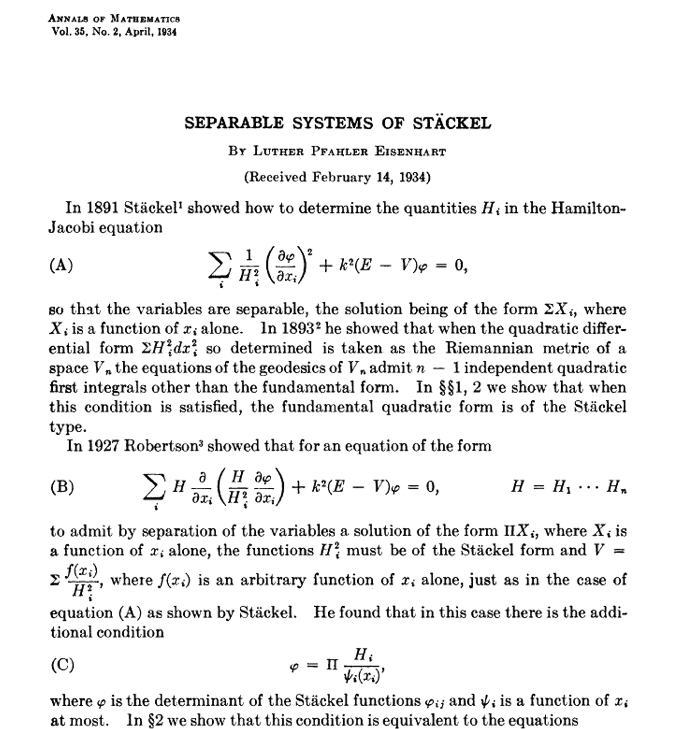
\includegraphics[scale=0.4]{Imagenes/Referencia_Eisenhart.png}
\end{figure}
\end{frame}
\begin{frame}
\frametitle{Referencias de consulta}
\begin{figure}
\centering
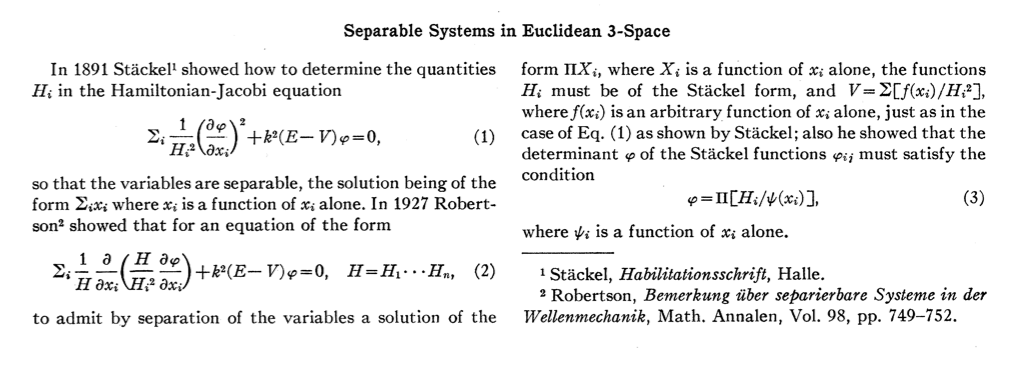
\includegraphics[scale=0.33]{Imagenes/Referencia_Eisenhart_02.png}
\end{figure}
\end{frame}
\begin{frame}
\frametitle{Referencias de consulta}
\begin{figure}
  \centering
  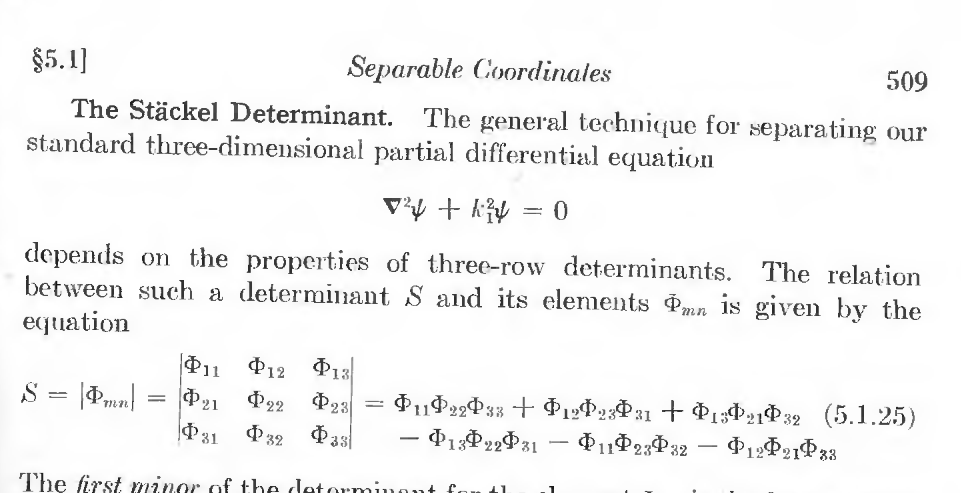
\includegraphics[scale=0.33]{Imagenes/Referencia_Morse.png}
\end{figure}
\end{frame}
\begin{frame}
\frametitle{La matriz $S$}
Para iniciar con la separación de variables, se hace uso de la matriz de Stäckel.
\end{frame}
\begin{frame}
\frametitle{La matriz $S$}
Cada sistema coordenado $u^{1}, u^{2}, u^{3}$, tiene asociada una matriz:
\pause
\begin{align}
[S] = \mqty[
\Phi_{11} \, (u^{1}) & \Phi_{12} \, (u^{1}) & \Phi_{13} \, (u^{1}) \\
\Phi_{21} \, (u^{2}) & \Phi_{22} \, (u^{2}) & \Phi_{23} \, (u^{2}) \\
\Phi_{31} \, (u^{3}) & \Phi_{32} \, (u^{3}) & \Phi_{33} \, (u^{3})
]
\label{eq:matriz_Stackel}
\end{align}
\pause
La principal característica de la matriz, es que cada renglón contiene funciones de una sola variable (o constantes)
\end{frame}
\begin{frame}
\frametitle{El determinante de Stäckel}
El determinante de Stäckel es el determinante de la matriz anterior (\ref{eq:matriz_Stackel}):
\pause
\begin{align}
S = \mqty|
\Phi_{11} & \Phi_{12} & \Phi_{13} \\
\Phi_{21} & \Phi_{22} & \Phi_{23} \\
\Phi_{31} & \Phi_{32} & \Phi_{33}
|
\label{eq:determinante_Stackel}
\end{align}
\pause
El objetivo del determinante de Stäckel, es determinar todos los elementos de la EDO, en la que es separable la ecuación tridimensional de Helmholtz.
\end{frame}
\begin{frame}
\frametitle{Cofactores del determinante}
Los cofactores de los elementos en la primera columna son:
\begin{align*}
M_{11} = \mqty|
\Phi_{22} & \Phi_{23} \\
\Phi_{32} & \Phi_{33}
| , \hspace{0.3cm}
M_{21} = -\mqty|
\Phi_{12} & \Phi_{13} \\
\Phi_{32} & \Phi_{33}
| , \hspace{0.3cm}
M_{31} = \mqty|
\Phi_{12} & \Phi_{13} \\
\Phi_{22} & \Phi_{23}
|
\end{align*}
\end{frame}
\begin{frame}
\frametitle{Condiciones necesarias}
Las condiciones necesarias y suficientes para una separación de la ecuación escalar de Helmholtz son:
\pause
\begin{equation}
\begin{aligned}
g_{ii} &= \dfrac{S}{M_{i1}} \\[0.5em] \pause
\dfrac{g^{\frac{1}{2}}}{S} &= f_{1} (u^{1}) \, f_{2} (u^{2}) \, f_{3} (u^{3})
\label{eq:ecuaciones_condiciones}
\end{aligned}  
\end{equation}
\end{frame}
\begin{frame}
\frametitle{Primera condición}
La primera condición:
\pause
\begin{align*}
g_{ii} = \dfrac{S}{M_{i1}}
\end{align*}
Establece la restricción para que sea posible construir el determinante de Stäckel y que está relacionada con los coeficientes métricos del sistema coordenado.
\end{frame}
\begin{frame}
\frametitle{La segunda condición}
La segunda condición:
\pause
\begin{align*}
\dfrac{g^{\frac{1}{2}}}{S} &= f_{1} (u^{1}) \, f_{2} (u^{2}) \, f_{3} (u^{3})
\end{align*}
La condición establece que la cantidad $\dfrac{g^{\frac{1}{2}}}{S}$ debe de ser separable.
\end{frame}
\begin{frame}
\frametitle{Ecuaciones separables}
Si ambas condiciones se satisfacen, las ecuaciones separables son:
\pause
\begin{align}
\dfrac{1}{f_{i}} \, \dv{u^{i}} \, \left( f_{i} \, \dv{U^{i}}{u^{i}} \right) + U^{i} \, \nsum_{j=1}^{3} \alpha_{j} \, \Phi_{ij} = 0
\label{ec:ecuacion_Helmholtz}
\end{align}
\pause
donde $i, j = 1, 2, 3$ y $\Phi_{ij}$ son los elementos de la matriz de Stäckel, $\alpha_{j}$ son las constantes de separación, con $\alpha_{1} = \beta^{2}$
\end{frame}
\begin{frame}
\frametitle{Las funciones $f_{i}$}
Para determinar las funciones $f_{i}$ nos apoyamos con la siguiente relación:
\pause
\begin{align*}
\dfrac{g^{\frac{1}{2}}}{g_{ii}} = f_{i} (u^{i}) \, h_{i}(u) \hspace{1.5cm} i = 1, 2, 3
\end{align*}
\pause
De esta manera ya podemos obtener el determinante $S$ a partir de:
\pause
\begin{align*}
S = \dfrac{f_{1} (u^{1}) \, f_{2} (u^{2}) \, f_{3} (u^{3})}{g^{\frac{1}{2}}}
\end{align*}
\end{frame}
\begin{frame}
\frametitle{Ortogonalidad de los determinantes}
Al considerar la ortogonalidad de los determinantes, podemos obtener los elementos de $\Phi_{ij}$, siempre que se cumpla la condición de separabilidad.
\end{frame}
\begin{frame}
\frametitle{Ecuaciones para los $\Phi_{ij}$}
Para $\Phi_{11}, \Phi_{21}, \Phi_{31}$, se tiene que:
\pause
\begin{align*}
M_{11} \, \Phi_{11} + M_{21} \, \Phi_{21} + M_{31} \, \Phi_{31} = S
\end{align*}
\pause
Para $\Phi_{12}, \Phi_{22}, \Phi_{32}$, se tiene que:
\pause
\begin{align*}
M_{11} \, \Phi_{12} + M_{22} \, \Phi_{22} + M_{31} \, \Phi_{32} = 0
\end{align*}
\pause
Para $\Phi_{13}, \Phi_{23}, \Phi_{33}$, se tiene que:
\pause
\begin{align*}
M_{11} \, \Phi_{13} + M_{22} \, \Phi_{23} + M_{31} \, \Phi_{33} = 0
\end{align*}
\end{frame}

\subsection{Ejemplo Coordenadas Esféricas}

\begin{frame}
\frametitle{Coordenadas Esféricas}
Expresa la ecuación de Helmholtz en el sistema coordenado esférico $(r, \theta, \varphi)$ mediante la matriz de Stäckel.
\end{frame}
\begin{frame}
\frametitle{Los factores de escala}
Sabemos que los factores de escala son:
\begin{align*}
g_{11}^{\frac{1}{2}} &= h_{r} = 1 \\[0.5em] 
g_{22}^{\frac{1}{2}} &= h_{\theta} = r \\[0.5em] 
g_{33}^{\frac{1}{2}} &= h_{\varphi} = r \, \sin \theta
\end{align*}
\end{frame}
\begin{frame}
\frametitle{Valores necesarios}
Podemos calcular entonces:
\pause
\begin{align*}
g^{\frac{1}{2}} = (g_{11} \, g_{22} \, g_{33})^{\frac{1}{2}} = r^{2} \, \sin \theta
\end{align*}
\pause
De tal modo que:
\begin{eqnarray*}
\dfrac{g^{\frac{1}{2}}}{g_{11}} = r^{2} \sin \theta \pause = f_{1}(r) \, g(u) \hspace{0.5cm} \Rightarrow \hspace{0.2cm} f_{1} = r^{2}
\end{eqnarray*}
\end{frame}
\begin{frame}
\frametitle{Los otros valores necesarios}
Para los otros dos cocientes:

\begin{eqnarray*}
\dfrac{g^{\frac{1}{2}}}{g_{22}} &=& \dfrac{r^{2} \sin \theta}{r^{2}} = \sin \theta \pause = f_{2}(\theta) \, g(u) \hspace{0.5cm} \Rightarrow \hspace{0.2cm} f_{2} = \sin \theta \\[0.5em] \pause
\dfrac{g^{\frac{1}{2}}}{g_{33}} &=& \dfrac{r^{2} \sin \theta}{r \, \sin \theta} = r \pause = f_{3}(\varphi) \, g(u) \hspace{0.5cm} \Rightarrow \hspace{0.2cm} f_{3} = 1
\end{eqnarray*}
\end{frame}
\begin{frame}
\frametitle{Calculando el determinante $S$}
Ya podemos calcular el determinante $S$:
\pause
\begin{align*}
S = \dfrac{g^{\frac{1}{2}}}{f_{r} \, f_{\theta} \, f_{\varphi}} = \dfrac{r^{2} \, \sin \theta}{r^{2} \, \sin \theta} = 1
\end{align*}
\pause
Así como los cofactores $M_{i1}$:
\pause
\begin{align*}
M_{11} = \dfrac{S}{g_{11}} = 1 \hspace{0.5cm} M_{21} = \dfrac{S}{g_{22}} = \dfrac{1}{r^{2}} \hspace{0.5cm} M_{31} = \dfrac{S}{g_{33}} = \dfrac{1}{r^{2} \, \sin^{2} \theta}
\end{align*}
\end{frame}
\begin{frame}
\frametitle{Los elementos $\Phi_{ij}$}
Ya contamos con lo necesario para calcular los $\Phi_{ij}$ de la matriz de Stäckel:
\begin{eqnarray*}
M_{11} \, \Phi_{11} + M_{21} \, \Phi_{21} + M_{31} \, \Phi_{31} &=& 1 \\[0.5em] \pause
(1) \, \Phi_{11} + \dfrac{1}{r^{2}} \, \Phi_{21} + \dfrac{1}{r^{2} \, \sin^{2} \theta}  \, \Phi_{31} &=& 1 \\[0.5em] \pause
\mbox{Los valores que satisfacen la expresión son:} \\[0.5em] \pause
(1) \, \Phi_{11} + \dfrac{1}{r^{2}} \, (0) + \dfrac{1}{r^{2} \, \sin^{2} \theta}  \, (0) &=& 1
\end{eqnarray*}
\end{frame}
\begin{frame}
\frametitle{Primeros elementos de $\Phi_{ij}$}
Entonces se tiene que:
\pause
\begin{align*}
\Phi_{11} = 1 \hspace{1cm} \Phi_{21} = 0 \hspace{1cm} \Phi_{31} = 0 
\end{align*}
\pause
La matriz de Stäckel va tomando la forma:
\pause
\begin{align*}
[S] = \mqty[
1 & \Phi_{12} & \Phi_{13} \\
0 & \Phi_{22} & \Phi_{23} \\
0 & \Phi_{32} & \Phi_{33}
]
\end{align*}  
\end{frame}
\begin{frame}
\frametitle{Los elementos $\Phi_{ij}$}
Luego entonces:
\begin{eqnarray*}
M_{11} \, \Phi_{12} + M_{21} \, \Phi_{22} + M_{31} \, \Phi_{32} &=& 0 \\[0.5em] \pause
(1) \, \Phi_{12} + \dfrac{1}{r^{2}} \, \Phi_{22} + \dfrac{1}{r^{2} \, \sin^{2} \theta}  \, \Phi_{32} &=& 0 \\[0.5em] \pause
\mbox{Los valores que satisfacen la expresión son:} \\[0.5em] \pause
(1) \, \left( - \dfrac{1}{r^{2}} \right) + \dfrac{1}{r^{2}} \, (1) + \dfrac{1}{r^{2} \, \sin^{2} \theta}  \, (0) &=& 0
\end{eqnarray*}
\end{frame}
\begin{frame}
\frametitle{Primeros elementos de $\Phi_{ij}$}
De donde tenemos:
\pause
\begin{align*}
\Phi_{12} = \left( - \dfrac{1}{r^{2}} \right) \hspace{1cm} \Phi_{22} = 1 \hspace{1cm} \Phi_{32} = 0 
\end{align*}
\pause
La matriz de Stäckel va tomando la forma:
\pause
\begin{align*}
[S] = \mqty[
1 & - \dfrac{1}{r^{2}} & \Phi_{13} \\
0 & 1 & \Phi_{23} \\
0 & 0 & \Phi_{33}
]
\end{align*}  
\end{frame}
\begin{frame}
\frametitle{Los elementos $\Phi_{ij}$ - 3}
Por último:
\pause
\begin{eqnarray*}
M_{11} \, \Phi_{13} + M_{21} \, \Phi_{23} + M_{31} \, \Phi_{33} &=& 0 \\[0.5em] \pause
(1) \, \Phi_{13} + \dfrac{1}{r^{2}} \, \Phi_{23} + \dfrac{1}{r^{2} \, \sin^{2} \theta}  \, \Phi_{33} &=& 0 \\[0.5em] \pause
\mbox{Los valores que satisfacen la expresión son:} \\[0.5em] \pause
(1) \, (0) + \dfrac{1}{r^{2}} \, \left( - \dfrac{1}{\sin^{2} \theta} \right) + \dfrac{1}{r^{2} \, \sin^{2} \theta} \, (1) &=& 0
\end{eqnarray*}
\end{frame}
\begin{frame}
\frametitle{Los últimos elementos de $\Phi_{ij}$}
Así completamos:
\pause
\begin{align*}
\Phi_{13} = 0 \hspace{1cm} \Phi_{23} = \left( - \dfrac{1}{\sin^{2} \theta} \right) \hspace{1cm} \Phi_{33} = 1 
\end{align*}
\pause
La matriz de Stäckel es:
\pause
\begin{align*}
[S] = \mqty[
1 & - \dfrac{1}{r^{2}} & 0 \\
0 & 1 & - \dfrac{1}{\sin^{2} \theta} \\
0 & 0 & 1
]
\end{align*}  
\end{frame}
\begin{frame}
\frametitle{Ecuaciones separadas}
De la ecuación:
\begin{align*}
\dfrac{1}{f_{i}} \, \dv{u^{i}} \, \left( f_{i} \, \dv{U^{i}}{u^{i}} \right) + U^{i} \, \nsum_{j=1}^{3} \alpha_{j} \, \Phi_{ij} = 0
\end{align*}
\pause
Con $\psi = R_{r} \, T_{\theta} \, F_{\varphi}$, con $f_{r}$:
\pause
\begin{align*}
\dfrac{1}{r^{2}} \, \dv{r} \left( r^{2} \, \dv{R}{r} \right) + R \bigg[ \beta^{2} + \alpha_{2} \left( - \dfrac{1}{r^{2}} \right) + \alpha_{3} (0) \bigg] = 0
\end{align*}
\end{frame}
\begin{frame}
\frametitle{La EDO separada}
La primera EDO2H separada para la ecuación de Helmholtz es:
\begin{align*}
\dfrac{1}{r^{2}} \, \dv{r} \left( r^{2} \, \dv{R}{r} \right) +  \beta^{2} \, R - \dfrac{\alpha_{2} \, R}{r^{2}} = 0
\end{align*}  
\end{frame}
\end{document}